\chapter{Android}\label{sec:Android}
This chapter will provide information about Android and Wear 2.0 technology. Why it was developed and what are the differences between previous version and other wear technologies.

\medskip

Android is a Linux based operating system for mobile and wear devices developed by Google. The main selling point of this system is that it's open-source project, meaning everyone can access the code and modify it as they wish. Android was mainly developed for mobile phones but in time moved beyond and at this time is implemented into all kinds of wear devices, tablets, televisions and even refrigerators or cameras.\cite{WIGA}

\section{Android system structure}\label{sec:AndroidSystemStructure}
Android is created as a stack, meaning there are functional modules stack on top of each other from Linux core over native libraries to applications as shown in \fref{fig6}. Android maintains complete software stacks to enable device creators to run and modify Android for their specific hardware. To support these modifications and testing every release has multiple "code lines" to separate stable versions from experimental work.\cite{AOSP}

\begin{figure}[H]
	\begin{centering}
		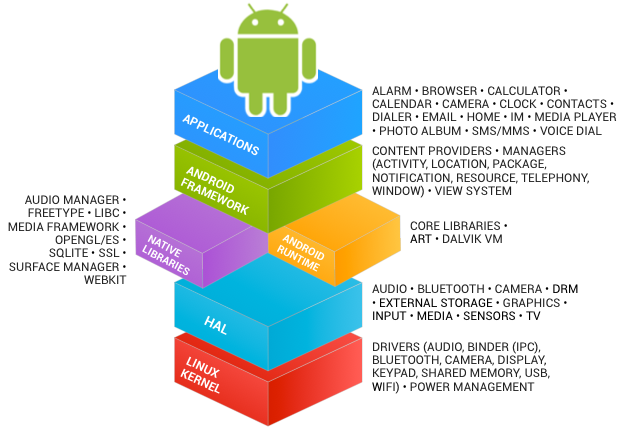
\includegraphics[width=0.6\textwidth]{img/android_stack}
		\par\end{centering}
	\caption{Android stack (source: \cite{AOSP})\label{fig:AndroidStack}}
	\label{fig6}
\end{figure}

There are multiple versions of Android system at this time and every single one has it's own version, code name and API level. Version codes are number identifications of a specific system version. Highest levels of these numbers are grouped into code names that are ordered alphabetically. As an example versions 8.0.0 and 8.1.0 have the same code name called Oreo. Finally API level is number identification for compatibility of specific application and it will be compared to API level of device Android system.\cite{AOSP}\cite{AD}

Android security...

\section{Wear technologies}\label{sec:WearTechnologies}
Interactive wearable, as an example smart watches, is a new part of mobile computers. Wear devices are categorically different from phones or tables in term of usage, design and user interfaces (UI). According to the app design guidelines by major vendors, users interact with wearable devices frequently throughout daily use. Each interaction is short, often less than 10 seconds, and is dedicated to simple tasks.\cite{UtCoAWO}

Important thing to note is that there are multiple kinds of wear devices from smart watches, wristbands, cameras or even glasses.\cite{MIWD} Based on report from Gartner technology research, conducted in 2017, most used wear devices were Bluetooth headset, wristbands and smartwatch. \cite{GSWWDS} Thanks to their small size wear devices are ideal to use for hands-free communication and health monitoring.

One problem with this diversity is hardware and software compatibility. Every device creator can create their own operating system for specific wear device and it can be difficult to develop custom applications for it. To bypass this problem this thesis is focused only on smartwatches with Android Wear operating system. 

\subsection{Android Wear}\label{sec:AndroidWear}
There are three main point to note with watch devices. First of all is small battery capacity that can be almost ten times smaller then in typical smart phone. The second point is smaller display with around forty-times less pixels which completely changes properties and also lovers the power consumption. And final part is scaled down CPU with high efficiency and lower power consumption.\cite{UtCoAWO}

\section{Other wear technologies}\label{sec:OtherWearTechnologies}
Pebble, Apple, Microsoft ...